\section{Testing e Verifica dell'Adeguatezza}

Il termine \textbf{testing} si riferisce all'eseguire un programma ed osservarne i risultati, andandoli a confrontare con un risultato atteso (si devono quindi avere delle specifiche). Bisogna inoltre definire quante volte è necessario eseguire l'operazione di testing (\textit{testing adequacy}). Un'altra, meno usata, definizione di testing si chiama ``exhaustive testing'', cioè che il sistema viene testato per tutti i possibili input. Vien da sè capire che questo tipo di testing è controverso, poiché non è possibile controllare tutti i possibili input (che sono infiniti, o comunque enormi). Questa controversia è riconducibile all'\textit{halting problem}: può esistere un algoritmo che risponde \textit{si} o \textit{no} rispetto alla terminazione di un programma qualsiasi? \textit{No}.

Quello che si ottiene attraverso la fase di testing è un'approssimazione ottimistica della qualità, ossia attraverso il test viene scelto un numero piccolo di tutti i possibili input (scelti in maniera intelligente). In particolare, si può ottenere: \begin{itemize}
    \item l'identificazione di un bug;
    \item le prove non manifestano bug (è ottimistico concludere che il programma funziona per tutti gli altri input)
\end{itemize}

\subsection{Terminologia dei bug (IEEE)}

Il termine \textit{bug} ha varie sfumature: \begin{itemize}
    \item failure; \\ osservazione del problema, ma non il codice che l'ha causato. In questa fase, ancora non si sa come correggere il problema
    \item fault; \\ si analizza il malfunzionamento, si analizza il codice, si evidenzia il problema e si comprende come correggerlo
    \item error; \\ ulteriore analisi del fault: ci si chiede il perché si è verificato l'errore, e di conseguenza ci permette di classificare i fault in base all'area in cui appartengono (es. errori di gestione della memoria, etc...)
\end{itemize}

\subsection{Selezionare il test a partire da una failure}

Come abbiamo detto in precedenza, non è possibile testare il software con tutti i possibili input. Come prima cosa, si fanno delle prove che vanno a stimolare il sistema in maniera mirata per trovare delle failure. Questo primo obiettivo è abbastanza intuitivo. Come seconda cosa, mano a mano che vengono eseguiti i test, che vengono identificati bug (e corretti), i pochi test rimasti da fare vano in convergenza. In pratica, una volta verificato che il software supera tutti i test previsti, ci si chiede \textit{``cosa sappiamo?''} In particolare, ci chiediamo se i test che abbiamo fatto siano sufficienti per poter definire il software di qualità e pronto al rilascio.

Le fasi, riassumendo, sono due: \begin{enumerate}
    \item effettuare prove intelligenti mirate alla risoluzione dei bug;
    \item verificare che le prove scelte nel punto precedente siano anche adeguate.
\end{enumerate}

\begin{example}[]{Simple game}
    Consideriamo la seguente applicazione sulla quale vogliamo eseguire dei test:

    \begin{figure}[H]
        \caption{Ciao}
        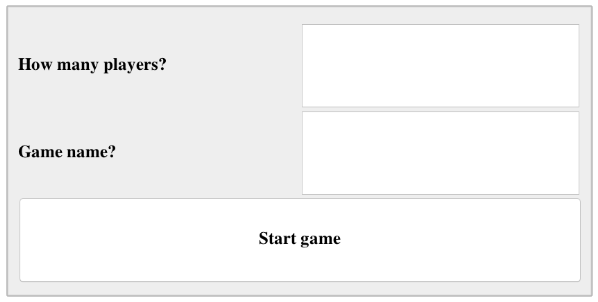
\includegraphics[width=\textwidth]{Lezioni/Lezione2/simplegame.png}
    \end{figure}
\end{example}